% Penn -> U.S. Dept. of Education / Default Resolution Group (FURNISHER direct dispute)
% Compile with XeLaTeX. Requires studentloan_core.tex and the exhibit PDFs in the same folder.
\documentclass[12pt,letterpaper]{article}
\usepackage[left=1.25in,right=1.25in,top=1in,bottom=1in]{geometry}
\usepackage{fontspec}
\usepackage{graphicx}
\usepackage{parskip}
\usepackage{enumitem}
\usepackage{titlesec}
\usepackage{booktabs}
\usepackage{array}
\usepackage{pdfpages}
\titleformat{\subsection}{\normalfont\bfseries\scshape}{\thesubsection}{1em}{}
\begin{document}

\begin{center}
  \textbf{VIA FACSIMILE AND CFPB PORTAL --- WRITTEN RECORD PRESERVED} \\
  \textbf{Date:} \underline{\today}
\end{center}

\begin{tabular}{@{}ll}
  \textbf{To:}   & U.S. Department of Education --- Federal Student Aid \\
                 & Attn: Richard Lucas, Chief Operating Officer, FSA \\
                 & and the Default Resolution Group \\
                 & P.O. Box 5609, Greenville, TX 75403-5609 \\
                 & \\
                 & \textit{cc:} Nicholas Kent, Under Secretary \\
                 & \hphantom{\textit{cc:} }Linda McMahon, Secretary \\
                 & \hphantom{\textit{cc:} }Office of the General Counsel \\
                 & \\
  \textbf{From:} & Ash Le' A. Penn \\
                 & 17548 NW Springville Rd \#9, Portland, OR 97229 \\
\end{tabular}
\vspace{1em}\hrule\vspace{1em}

\textbf{Borrower:} Ash Le' A. Penn (``Consumer''/``Borrower'') \\
\textbf{Social Security No.:} XXX-XX-7755 \quad \textbf{DOB:} 02/15/1988 \\
\textbf{Loan Program:} William D. Ford Federal Direct Loans \\

\begin{center}
  \textbf{Re: Formal Direct Dispute (FCRA \S~1681s-2(a)(8) / 12 C.F.R. \S~1022.43); \\
    Privacy Act Request to Amend (5 U.S.C. \S~552a(d)); \\
    Demand for Documentation}
\end{center}

\vspace{1em}
\textbf{Attached Exhibits:}
\begin{enumerate}[noitemsep]
  \item Valid State-Issued ID \& Current Utility Bill
  \item Equifax report 09/24/2024
  \item Equifax report 03/01/2026
  \item Master Promissory Note (¶20 highlighted)
  \item TransUnion Credit Report dated 03/01/2026 (showing expired removal dates)
  \item A copy of this dispute
\end{enumerate}
\vspace{1em}\hrule\vspace{1em}

To Whom It May Concern:

This is a formal direct dispute of the accuracy and completeness of the information the U.S. Department of Education, its servicer Nelnet, and its Default Resolution Group (collectively, ``the Department'') have furnished to the nationwide consumer reporting agencies regarding the Consumer's federal Direct Loans, submitted under FCRA \S~1681s-2(a)(8) and 12 C.F.R.\ \S~1022.43, as a Privacy Act request to amend agency records under 5 U.S.C.\ \S~552a(d), and as a demand for documentation. It is submitted in good faith and is not frivolous under 12 C.F.R.\ \S~1022.43(f). \textbf{Nothing herein is an admission or reaffirmation of any debt; the Consumer reserves all rights.}

\input{studentloan_core.tex}

\subsection*{Demands}
\begin{enumerate}[label=\arabic*., leftmargin=*]
  \item Substantiate the Date of First Delinquency the Department is reporting (10/06--11/05/2024) by producing the complete account payment ledger and identifying the payment relied upon to advance it. Absent that substantiation, delete the tradelines as inaccurate and obsolete under \S~1681c(a).
  \item Substantiate the reported ``Date of Last Payment'' of 08/06/2023 with proof of an actual payment, or correct and delete it.
  \item Produce dated proof of the MPN ¶20 thirty-day advance notice and review opportunity, with proof of mailing/delivery, and of any \S~1681s-2(a)(7) notice.
  \item Reconcile the ten collection tradelines against the nine originating loans and delete any collection tradeline without a corresponding loan.
  \item Respond in writing within 30 days.
\end{enumerate}

\subsection*{Reservation of Rights}
Nothing herein waives any right or remedy, including FCRA \S\S~1681n and 1681o (willful and negligent noncompliance), which apply to the Department as a federal agency per \emph{Dept.\ of Agriculture Rural Development Rural Housing Service v.\ Kirtz}, 601 U.S.\ 42 (2024); FCRA \S~1681h(e); FCRA \S~1681i and \S~1681s-2(b) via the Consumer's parallel disputes to the bureaus; the Higher Education Act; the Privacy Act, 5 U.S.C.\ \S~552a; and the Debt Collection Act, 31 U.S.C.\ \S~3711.

\vspace{1.5em}\noindent Respectfully, \\ \vspace{1em}
\noindent 
\includegraphics[width=2.5in]{signature.jpg} \\
\textbf{Ash Le' A. Penn}

\newpage \includepdf[pages=-]{ID.png}
\newpage \includepdf[pages=-]{Proof_of_Address.pdf}
\newpage 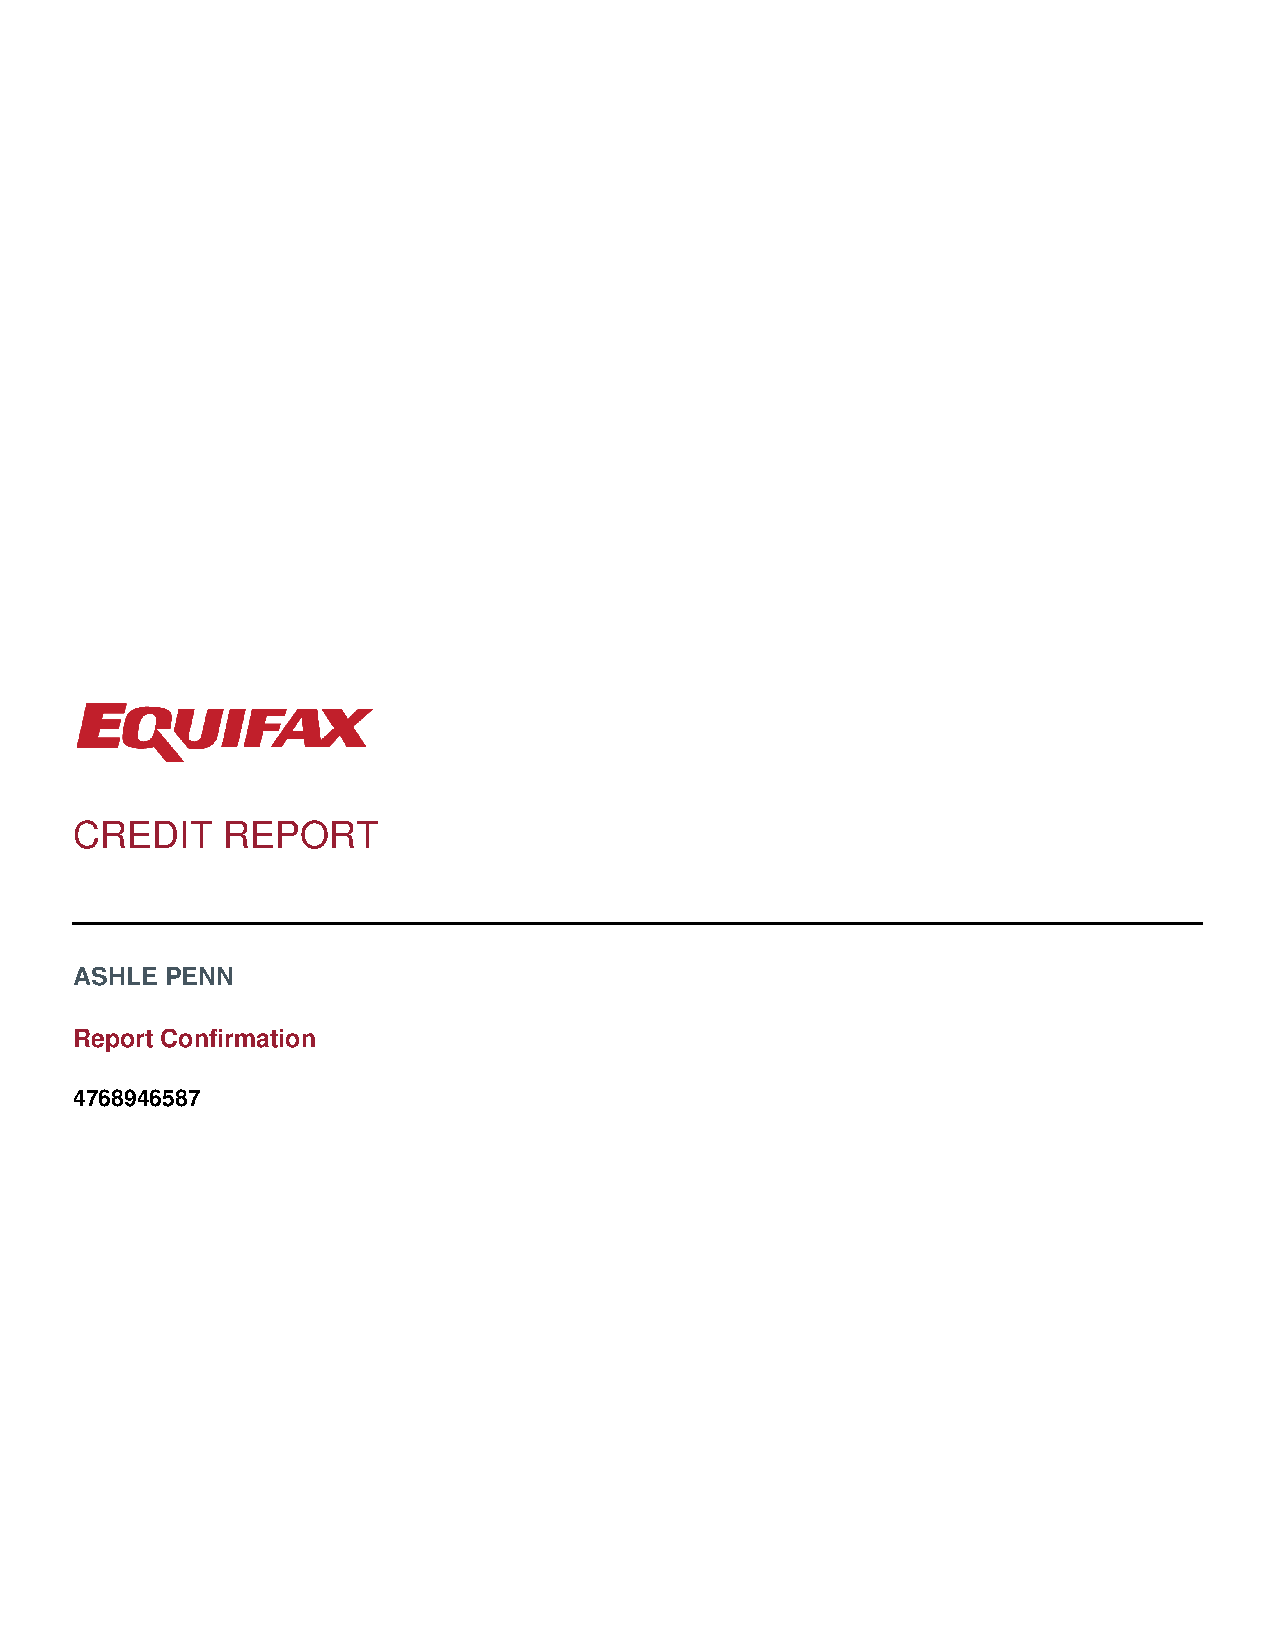
\includepdf[pages=-]{EQUIFAX_9.24.24.pdf}
\newpage \includepdf[pages=-]{EQUIFAX_3.1.26.pdf}
\newpage \includepdf[pages=-]{MPN.pdf}
\newpage \includepdf[pages=-]{TransUnion Credit Report.pdf}
\end{document}
